\section{Driver in the FPGA}
This section describes how the driver is implemented in the FPGA. The section starts with an overall analysis of the system and afterwards goes into details with some blocks defined in the analysis and ends with a discussion on how the PID controller could have been implemented better as a filter.

\subsection{Overall analysis}

The easiest way to describe how the overall system works is by looking at the general components and how they are connected. The general components used in the implementation are: a comparator, a controller, a sensor, a motor driver with a PWM module and a SPI slave with a data bank. A generic multiplexer display was also added to simplify the debugging process, however this should not be seen as a part of the final product.
Since the goal is to control two motors a separate controller setup was made for each motor. This means that each motor is connected to its own setup of a comparator, a sensor, a controller and a motor driver. The SPI slave component is common for the motors.
Figure \ref{fig:IDEA_WEIGHT_v2} is an illustration of how the components are internally connected. This figure also shows information on the signals between the individual components.

\newpage
\begin{figure}[h!]
\centering
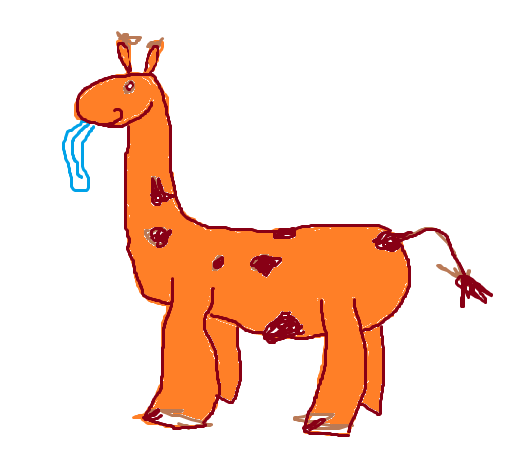
\includegraphics[scale=0.5]{billeder/IDEA_WEIGHT_v2.png}
\caption{ Placeholder figure }
\label{fig:IDEA_WEIGHT_v2}
\end{figure}
\newpage

The components can be divided into the following blocks, each with a specific purpose. 

\textbf{The first block} is the SPI slave block which contains only the SPI slave component. The purpose of this block is to receive and store information used by the rest of the components. It then shares the information with the components that are in need of them. An example of this could be the maximum and minimum speed of a motor which is sent to the controller (this connection can also be seen on figure \ref{fig:IDEA_WEIGHT_v2}.

\textbf{The second block} is the controller block which contains the comparator and the controller components. The purpose of this block is to regulate the motors according to a target input and the feedback. The block generates a duty cycle and a direction that is passed onto the motor driver.

\textbf{The third block} is the sensor block which consists only of the sensor component. The purpose of this block is to keep track of the current position of the motor. This is done by looking at the hall sensors from the motors and relating their output to the current position.

\textbf{The last block} is the motor driver which contain the motor driver component and its internal PWM module. The purpose of this block is to control and power the motor. This means that the block generates a PWM signal and outputs it on the correct pin according to the desired direction.

